\documentclass{article}
\usepackage{amsmath}
\usepackage{amssymb}
\usepackage{graphicx}
\usepackage{hyperref}
\usepackage[version=4]{mhchem}


\begin{document}
Show that the measure of the median on the hypotenuse of a right triangle is one-half the measure of the hypotenuse ( \(A M\) \(=M B=M C\) ).

Proof:
Extend \(C M\) to \(D\) such that \(C M=D M\).\\
\centering
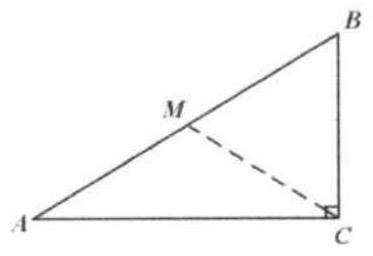
\includegraphics[width=\textwidth]{images/024(2).jpg}

Connect \(B D\) and \(A D\).\\
\(A B\) and \(C D\) are two diagonals and they bisect each other. So \(A C B D\) is a parallelogram.

Since \(\angle C=90^{\circ}, A C B D\) is a rectangle.\\
\centering
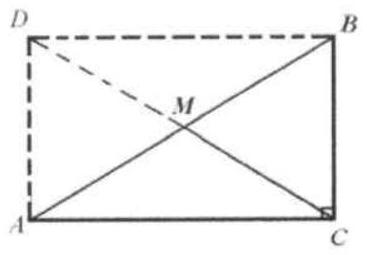
\includegraphics[width=\textwidth]{images/024(1).jpg}

Thus \(D M=M C=A M=M B\).


\end{document}
